\documentclass[10pt]{article}
\setlength{\textwidth}{6.3in}
\setlength{\textheight}{9in}
\setlength{\oddsidemargin}{0in}
\setlength{\evensidemargin}{0in}
\setlength{\topmargin}{-.5in}
%\parindent=0in
\linespread{1.3}
\usepackage{ mathrsfs }
\usepackage{amsthm}
\usepackage{ amssymb }
\usepackage{graphicx}
\newtheorem{theorem}{Theorem}[section]
\newtheorem{lemma}[theorem]{Lemma}

\usepackage{amsmath}
\usepackage{amsfonts}
\usepackage{fancyhdr}
\pagestyle{fancy}
\headheight = 14.5pt
\lhead{Probability HW7, Thomas Zeng }
\rhead{Math 240, Fall 2022}
\cfoot{\thepage}

\begin{document}
\section*{1}
%6.4
\subsection*{a}
We want $P(X\ge12)=1-F(12) = 1 - (1-\exp(-0.03(12)^{1.2}))\approx0.55.$

\subsection*{b}
\begin{align*}
    f(x) &= F(x)\frac{d}{dx}\\
    &= 1-\exp(-0.03x^{1.2})\frac{d}{dx}\\
    &=0.03(1.2)\exp(-0.03x^{1.2})x^{.2}\\
    &= 0.036\exp(-0.03x^{1.2})x^{.2}
\end{align*}
\noindent
(implicitly $f(x)=0$ if $x\le0$)

\section*{2}
%6.16
We define $X\sim\text{Exp}(\frac{1}{5})$ where $X$ represents the number of minutes before the next text.
\subsection*{a}
We want $Pr(X>10)=1-Pr(X\le10)\approx0.14$ using \texttt{1-pexp(10,1/5)}.
\subsection*{b}
We want $Pr(X\le10) - Pr(X\le7)\approx0.11$ using \texttt{pexp(10,1/5)-pexp(7,1/5)}.
\subsection*{c}
We want $Pr(X<3)=Pr(X\le3)\approx0.45$ using \texttt{pexp(3,1/5)}.
\subsection*{d}
Exponential distribution is memoryless so $Pr(X>7|X>5)=Pr(X>2)=1-Pr(X\le2)\approx0.67$ using \texttt{ 1-pexp(2,1/5)}.

\section*{3}
%6.20
\subsection*{a}
$Pr(X<18)=Pr(X\le18)\approx0.59$ using \texttt{pexp(18,1/20)}.
\subsection*{b}
$Pr(X\le23)-Pr(X<15)=Pr(X\le23)-Pr(X\le15)\approx0.16$ using \texttt{pexp(23,1/20)-pexp(15,1/20)}.\
\subsection*{c}
$Pr(X\ge26)=1-Pr(X<26)=1-Pr(X\le26)\approx0.27$ using \texttt{1-pexp(26,1/20)}

\section*{4}
%6.22
\subsection*{a}
\begin{align*}
    \int_0^m\lambda e^{-\lambda x}dx &= \frac{1}{2}\\
    -e^{-\lambda x}\Bigr |_0^m &= \frac{1}{2}\\
    -e^{-\lambda m}+1&=\frac{1}{2}\\
    e^{-\lambda m} &= \frac{1}{2}\\
    -\lambda m &= \ln\frac{1}{2}\\
    m&=-\frac{\ln 0.5}{\lambda}
\end{align*}

\subsection*{b}
\begin{align*}
    \mu-m&=\frac{1}{\lambda} - (-\frac{\ln 0.5}{\lambda})\\
    &= \frac{1+\ln0.5}{\lambda}\\
    &> 0 \quad \text{as } \ln 0.5 \approx -0.69<1
\end{align*}

The difference is positive, and thus the mean is larger than the median.

\section*{5}
%7.2
\subsection*{a}
$Pr(|X|<2)=Pr(-2<X<2)=Pr(X\le2)-Pr(X\le-2)\approx0.16$ using \texttt{pnorm(2,4,2)-pnorm(-2,4,2)}.
\subsection*{b}
$Pr(e^X<1)=Pr(X<\ln 1)=Pr(X\le0)\approx0.023$ using \texttt{pnorm(0,4,2)}.
\subsection*{c}
$Pr(\sqrt{X}>3)=Pr(X<-\sqrt{3}) + Pr(X>\sqrt[]{3})=1-Pr(X\le\sqrt[]{3})+ Pr(X\le-\sqrt[]{3})\approx0.87$ using \texttt{1-pnorm(3\string^0.5,4,2)+pnorm(-3\string^0.5,4,2)
}.
\section*{6}
%7.6
The SAT distribution is $X\sim\text{Norm}(500,100).$
With a score of $680$ this is the 0.96 quantile using \texttt{pnorm(680,500,100)}.

The ACT distribution is $Y\sim\text{Norm}(18,6).$ Thus, in order for Wyatt to be in the same quantile, he must score $28.8$ using \texttt{qnorm(pnorm(680,500,100),18,6)}.

\section*{7}
%7.26.ac To do later
\subsection*{a}
This is proportional to a normal distribution where $\mu=-1$ and $\sigma=3$ as $$e^{-(x- (-1))^2/(2\times3^2)}=e^{-(x+1)^2/18}.$$ We thus have
\[\int_{-\infty}^{\infty}\frac{1}{3\sqrt{2\pi}}e^{-(x+1)^2/18}dx=1\]
Thus the integral 
\[\int_{-\infty}^{\infty}e^{-(x+1)^2/18}dx\]
will be equal to $$\sigma\sqrt[]{2\pi}=3\sqrt{2\pi}.$$

\subsection*{c}
This is proportional to a gamma distribution with $\lambda=2$ and $a=5$ as $$x^{5-1}e^{-2x}=x^{4}e^{-2x}.$$ Thus
\[\int_{-\infty}^\infty\frac{\lambda^a}{\Gamma(a)}x^{4}e^{-2x}dx=\int_{-\infty}^\infty\frac{2^5}{(5-1)!}x^{4}e^{-2x}dx=1\]
and hence the integral will be \[\left (\frac{\lambda^a}{\Gamma(a)}\right )^{-1} =\left (\frac{2^5}{(5-1)!}\right )^{-1}=0.75.\]

\section*{8}
%7.34
\subsection*{a}
\begin{align*}
    \int_0^1cf(x)dx&=1\\
    \int_0^1cx^5(1-x)dx&=1\\
    c\int_0^1x^5-x^6dx&=1\\
    c\left (\frac{x^6}{6}-\frac{x^7}{7}\right )\Bigr |_0^1&=1\\
    c(\frac{1}{6}-\frac{1}{7})&=1\\
    c&=42
\end{align*}
\subsection*{b}
From the pdf, we have that $a=6$ and $b=2.$ Thus $E[X]=\frac{6}{6+2}=\frac{3}{4}$ and $V[X]=\frac{6\times2}{(6+2)^2(6+2+1)}=\frac{1}{36}.$
\subsection*{c}
$Pr(X<0.4)=Pr(X\le0.4)\approx0.019$ using \texttt{pbeta(0.4,6,2)}.

\section*{9}
\subsection*{a}
If we plot $F_X$ using Mathematica,
\begin{verbatim}
    Plot[Piecewise[{{0, x <= 0}, {2*x/5,1 >=x > 0},{(x^2 + 1)/5,2>=x>1},{1, x>2} }], {x, -2, 5}]\end{verbatim}
    we get a plot like the following.
    \begin{center}
        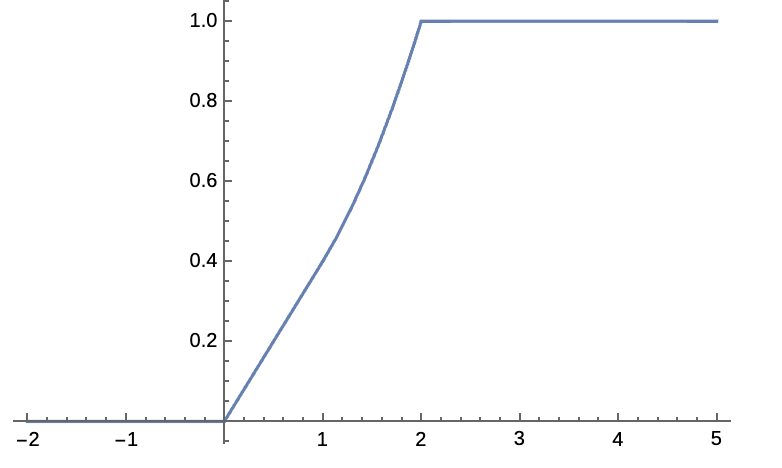
\includegraphics[width=0.5\textwidth]{hw7_9.png}
    \end{center}

Clearly this is non-decreasing, right continuous, and $F(-\infty)=0, F(\infty)=1.$ Thus, it satisfies the properties of a CDF for an RV.
\subsection*{b}
We know that $f(x)=F_X(x)\frac{d}{dx}$.
Thus, we have
\begin{equation*}
    f(x)=\begin{cases}
        0\frac{d}{dx}, \; x\le0\\
        2x/5\frac{d}{dx}, \; 0<x\le1\\
        (x^2+1)/5\frac{d}{dx}, \; 1<x\le 2\\
        1\frac{d}{dx}, \; x>2
    \end{cases}
\end{equation*}
If we take the derivative, we get
\begin{equation*}
    f(x)=\begin{cases}
        0, \; x\le0\\
        \frac{2}{5}, \; 0<x\le1\\
        \frac{2x}{5}, \; 1<x\le 2\\
        0, \; x>2
    \end{cases}
\end{equation*}
\subsection*{c}
$P(X<0.5)=F_X(0.5)=2(0.5)/5=0.2$
\subsection*{d}
$P(0.5<X<1.5) = F_X(1.5)-F_X(0.5) = (1.5^2+1)/5-0.2=0.45$
\subsection*{e}
\begin{align*}
    E[X] &= \int_{-\infty}^\infty xf(x)dx\\
    &= \int_0^1x\frac{2}{5}dx + \int_1^2x\frac{2x}{5}dx\\
    &= \frac{x^2}{5}\Bigr |_0^1 + \frac{2x^3}{15}\Bigr |_1^2\\
    &= \frac{1}{5} + \frac{16}{15} - \frac{2}{15}\\
    &= \frac{17}{15}
\end{align*}

\section*{10}
\subsection*{a}
Let $X\sim\text{Norm}(580, 70^2)$ be the distribution of SAT scores.
Then we have $Pr(\text{score $650$ or higher})\approx 0.159$ using \texttt{1-pnorm(650,580,70)}.

Now let $Y\sim\text{Geom}(0.159)$ be the probability of picking someone with a score of $650$ or higher. Then $Pr(Y=1)=0.159.$

\subsection*{b}
The probability of choosing $3$ with lower than $650$ and $2$ with $650$ or higher is $(1-0.159)^3(0.159)^2.$ There is $\binom{5}{2}$ ways this can be done. Thus the probability is $\binom{5}{2}(1-0.159)^3(0.159)^2\approx0.15.$

\section*{11}
We have $Pr(Y=y) = Pr(X=y/100)$. Thus the pdf is $f(y)=\frac{\Gamma(a+b)}{\Gamma(a)\Gamma(b)}(y/100)^{a-1}(1-y/100)^{b-1}/100$ using the chain rule. This is on the interval $0<y/100<1$ or $0<y<100$ and the value of $f$ is $0$ o.w. 
\end{document}